%%%% ijcai11.tex

\typeout{IJCAI-13 Instructions for Authors}

% These are the instructions for authors for IJCAI-13.
% They are the same as the ones for IJCAI-11 with superficical wording
%   changes only.

\documentclass{article}
% The file ijcai13.sty is the style file for IJCAI-13 (same as ijcai07.sty).
\usepackage{ijcai13}

% Use the postscript times font!
\usepackage{times}

% the following package is optional:
\usepackage{latexsym} 

% Algorithm package
\usepackage{algorithm}
\usepackage{algorithmic}
\usepackage{pgffor}

% Graphics package
\usepackage{graphicx}

% Following comment is from ijcai97-submit.tex:
% The preparation of these files was supported by Schlumberger Palo Alto
% Research, AT\&T Bell Laboratories, and Morgan Kaufmann Publishers.
% Shirley Jowell, of Morgan Kaufmann Publishers, and Peter F.
% Patel-Schneider, of AT\&T Bell Laboratories collaborated on their
% preparation.

% These instructions can be modified and used in other conferences as long
% as credit to the authors and supporting agencies is retained, this notice
% is not changed, and further modification or reuse is not restricted.
% Neither Shirley Jowell nor Peter F. Patel-Schneider can be listed as
% contacts for providing assistance without their prior permission.

% To use for other conferences, change references to files and the
% conference appropriate and use other authors, contacts, publishers, and
% organizations.
% Also change the deadline and address for returning papers and the length and
% page charge instructions.
% Put where the files are available in the appropriate places.

\begin{document}

\title{Atom based Adaptive Multi Dimensional Motif Discovery\thanks{These match the formatting instructions of IJCAI-07. The support of IJCAI, Inc. is acknowledged.}}
%\author{ Yu Chen \qquad Joshua Shinavier \qquad James Hendler \qquad Peter Fox \\ %Tetherless World Constellation \\
%Rensselaer Polytechnic Institute \\
%Troy NY, 12180 \\
%\texttt{$\lbrace$cheny18,pfox$\rbrace$@cs.rpi.edu}
%}
% Arrangement: 
% Abstract and Introduction: Page 1
% Related Work: Page 1-2
% Motivation: Page 2
% Motif detecton algorithm: Page 3
% Motif detectoin alg via aggregation: Page 4
% Multi-dimensional with linear kernel: Page 4
% Experiment: Page 5
% Discussion and Conclusion: Page 6
% Reference: Page 6
\maketitle

\begin{abstract}
  {    Motif discovery has been an important approach in aggregating and understanding complex 
	time series data in the field of bioinformatics, signal processing and event detection. However, 
	supervision and domain knowledge are necessary to find the most appropriate motif. The problem 
	can be much tougher while conducting multi-dimensional motif detection as the time series data 
	in each dimensional has their own characteristics. In this paper, we proposed and experimented with 
	a new algorithm that can find the most appropriate multi-dimensional motif automatically. To demonstrate the advance of the algorithm, 
	we experiment with handheld sensor data and data from public data repository. The result shows that 
	our algorithm works perfectly on finding the multi-dimensional motif while still guaranteeing a linear 
	timing complexity. 
	}
\end{abstract}

\section{Introduction}

This paper addresses the problem of unsupervised event detection from time-series data. The data include but not limited to the ones from wearable mobile sensors, scientific environmental monitoring sensors, public surveillance sensors and tendency of the stock price etc. Activities and events can be represented as certain recurring patterns, or $motifs$ in the time series. $Motifs$ are set of subsequences recurring frequently in time-varying data. The goal of this work is to discover the the multi-dimensional motifs without human supervision or domain expertise. The problem is not trivial since we know nothing about the length, shape, frequency or positions of the motifs in prior. We don't even know if there is one existed. Furthermore, as the data is collected from real-world, we must be able to deal with the noise, jitter and delay hidden in the time series. Last but not least, the algorithm must be efficient enough to extract the motifs from various sensor data sources. Therefore, the algorith must be linear or pseudo-linear in time complexity to meet the requirement in real application scenario. 

The motivation for our work is based on Atomism, a natural philosiophy proposed by Robert Boyle. It argues that the natural world is constructed by fundamental parts: indivisible atoms and empty voids. Although recent research shows that atoms can further decompose to more fundamental elements, the idea of arranging fundamental components organically to construct a giant functioning parts is profound. Therefore, we adopt the idea and experience from this basic theorem and apply similar tricks to boost the performance of the motif detection algorithm. 

Our contributions in this paper are as following: (1) Defined a metric in evaluating motif detection algorithm(2) Completely remove the configuration required of user(3) Improved the accuracy and time complexity of the exact motif discovery algorithm. (4) Extended the applicability of the algorithm in real world multi-dimensional motif detection scenario. Section ?? briefly overviewed the general workflow of motif detection algorithm. Section ?? explains in detail the motivation and idea behind the algorithm. Section ?? demonstrate the advance of the algorithm theoretically. Section ?? shows the experiment results performed by our algorithm in comparison with others. Section concludes the paper with some discussion and future works. 

\section{Background and Related Work}
Motif discovery has been an active research topic in event detection, context modeling and bioinformatics etc. Many efforts has been done on the motif discovery of time-varying data. One of the approaches is based on the work of Keogh and colleages \cite{Lin03asymbolic} in which motif is discovered in comparing euclidean distance between frequently appreared seed sliding windows after transforming the real-valued time series to symbolic strings.\cite{Lin03asymbolic} firstly propose the approach to use symbols to represent the time varying data. The continuous time series data will therefore be represented as a string of discrete characters where each represent the relative value compared to the other data after normalization. \cite{Chiu03probabilisticdiscovery} later introduce the probalistic random projection to find the motifs in sub-quadratic time. The approach is to use fixed-size sliding window along the the symbolic strings assuming the motif will just fit each window. Then the motifs will be arranged as rows in a matrix. The random projection algorithm works by randomly select two columns for all the sliding windows; if two sliding windows happens to have the same value on those two columns, we can argue that these two sliding windows contain the same symbolic string for a high probability and therefore we add one to the entry in the motif collision table. The random project will be conducted for several times, but significanty less than the length of the sliding window. Later, a pair of sliding windows whose corresponding table entries is above a certain threshold $T$ will be regarded as the same motif. These pairs of motif will be regarded as seeding motif. Then the algorithm go over every time series corresponding to a sliding window; for each time series window, if the minimum of the euclidean distance to those seeding motifs is below a threshold $R$, it will also be regarded as the same motif as the seeding ones. In this way, we can extract the motifs in a univariate time series. One of the recent work is from \cite{Mueen09exactdiscovery} in which the threshold value is calculated using second derivatives and thus remove the burden from user's in choosing a domain specific threshold parameter. However, this work does not consider the case when motifs in time series are with different length. Another approach tries to find high density regions of each subsequences through clustering. Some of the representative works are from \cite{Minnen:2007:DMM:1619645.1619744} where they encode the motif as a vector using the mean and variance value within a window length. However, the user still need to configure a proper window size as one vital parameters to the algorithm. The choice for the window size is crucial in determining whether the motif obtained will just be the one as we expected. Nevertheless, this choice is very tricky and needs to be tuned several times even for domain expertes. Therefore, the algorithm can not be left running unsupervised especially in terms of large scales of sensor data streams from sensors of different specifications. The ideas of using short motifs to construct large motifs is mentioned at \cite{Saria:2011:DDM:2283516.2283640} which we got inspired to develop an absolute unsupervised motif discovery algorithm. 

In terms of multi-dimensional motif discovery, one of the recent work is \cite{Vahdatpour09towardunsupervised} in which they use a graph model to calculate the correlation between motifs in different dimension. However, the model is not applicable to real cases where delay and jitter of the time series data occur and therefore not noise-tolerant. The problems discussed above will be addressed in the following sections of our work. 

\section{Motivation}
In the current research in motif detection, it is always a tricky problem to select the most appropriate window size. The proper window size
is the key to discover the most appropriate motif within one time series data. However, this requires domain expertise as 
well as sometimes looking at the data. Otherwise, few motif will be detected or partial motifs are obtained, which all suppress the prossibility 
for further multi-motif detection or event recognition. Therefore, it is vital to develop a adaptive algorithm to find the most
appropriate motifs within the time series data. Here we define the most appriate motifs within the time series $T$ as the frequently appeared motifs 
set $MTL$ such that it covers the maximum of time series data while containing the least number of different motifs. Assume the percetage of the 
time series that is covered by all the motifs is $PCT(MTL,T)$ and the number of different motifs is $SetSize(MTL)$, then the index that evaluating 
the performance of the motif discovered is $Index = PCT(MTL,T)/SetSize(MTL), index \in (0,1)$. The goal is to maximize the $index$. 
Since motif is defined as the subsequences that appeared more than once within a time series, the trivial maximum where the whole time series act as a 'subsequence', i.e. $PCT(MTL,T)=1,SetSize(MTL)=1$ can never happen. 

Now that we have a criteria in evaluating the performance of the algorithm, the approach is simply to maximize the percentage that the motif covers the 
time series while at the same time, minimizing the number of different motifs. In previous works, the basic assumption before conducting motif discovery algorithm 
is the length of motifs within one time series is the same. While this is a good initial approach in motif detection, it is nevertheless an assumption that ignore the fact that 
a single time series data could contain various information from different perspectives. For example, the data produced by wearable accelerometer can reflect human's motion 
such as walking, running, standing up, sitting down. Not all of them are with the same motif length. Therefore, the assumption that motif are with the same length does not fit into real scenarios. 

So how to detect the motif with different length within a single time series? This is the problem we tackled. Bearing in mind that long motifs are constructed by short motifs, once 
we have all the short motifs, we can merge the short motifs if they always happen around the same time with a specific sequencing pattern. Based on this idea, we come up with 
the algorithm of Automatic Motif Discovery via Aggregation, which will be further discussed in the following sections. 

\section{Automatic Motif Discovery via Aggregation}
We propose a new approach in discovering the actual motif by aggregating short base-motifs. 
Initially, we apply the SAX algorithm to convert the time series data to symbolic strings. 
The sliding window size should be relatively small in order to capture the subtle change of the time 
series data. After we obtain the symbolic string, we apply random projection using a relatively 
small window size, again to guarantee the shortest motif can be captured. 

% Needs to have motif collision table here
\begin{figure}
  \centering
  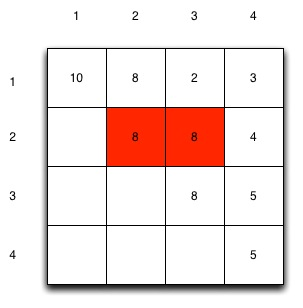
\includegraphics[scale=0.3]{BCT}
  \caption{Base Motif Collision Table}
\end{figure}

Now that we have a set of base-motifs, we need to construct the motif collision table to record if those base-motif overlapps. 
This collision table is vital in evaluating if several base-motifs should be aggregated to longer motifs. 
Let's assume there are N different base-motifs found by random projection. Then an $N \times N$ Base-motif Collision Table(BCT)
will be constructed while each entry BCT(i,j) represents the number of collisions between motif with id i and j. 
This algorithm basically go through all the motifs and check if two motifs overlap with each other. If they do, 
the entry BCT(i,j) will be added one. Finally, we obtain an upper-triagular matrix that reflects the collision between those motifs. 

 The algorithm picks the first appeared base-motif in the sequence and checks those 
overlapped with this base-motif: if the number of collisions between two base-motifs is the same as the number of occurance of the motif accroding 
to BCT, then we can argue these two motifs happens at around the same time, and they should be merged together. 
Then the algorithm take record of the ids that had been merged to this one. This is to avoid merging the motifs with the same id twice. 
The algorithm also store the starts and ends of the motif that had been merged in order to calculate the starts and ends of the new motif.
 A recursive call will be conducted with respect to the collided motifs to find the motif co-occur with the base-motif just being merged. 
The recursive call will return all the starts and ends of the motifs to be merged. Then we form the new motif by picking the smallest starts and largest ends as the starts and ends.  The time complexity of this algorithm is $O(n)$ where n is the number of motifs. 

\begin{figure}
  \centering
  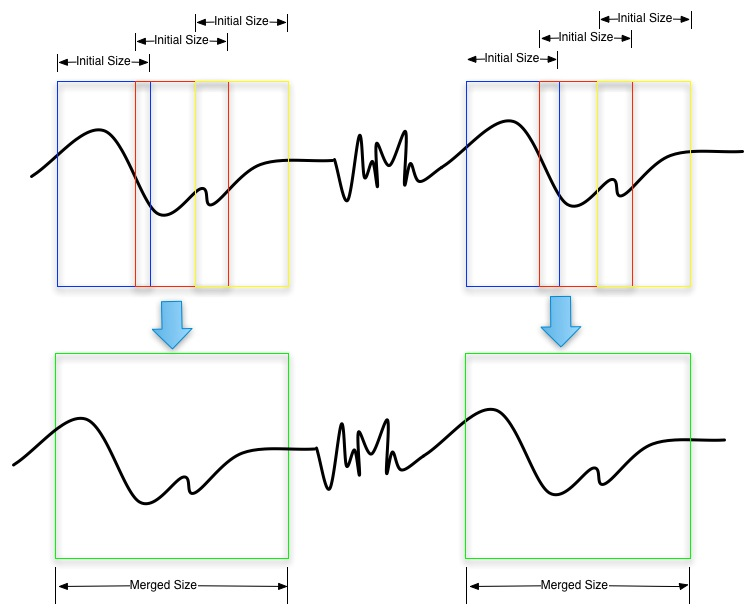
\includegraphics[scale=0.3]{MotifMerge}
  \caption{Merge sub-motif into the most appropriate motif}
\end{figure}

Let's assume the M is the set of all the motifs discovered using the random projection algorithm. The motifs that had been merged to the new motif will be removed from M to avoid re-calculation.Assuming the $CM$ is the motif that is checked on merging,$M.top$ is the first appeared motif in the time sequence, $CLSM$ is the set of id for all the collided motifs w.r.t $CM$, $NML$ to be the matrix that contains the new motifs after merging, $MM$ to be the merged motifs, $MBM$ to be the function that Merge Base-Motifs(MBM) to real motifs and Find Merged Motif Recurison($FMMR$) to be the recursive function that return the merged motifs. 

The pseudocode is shown as below:

\begin{algorithm}
\caption{MBM}
\begin{algorithmic} 
\WHILE{$M \neq \emptyset$}
\STATE $ CM \leftarrow M.top$
\STATE $ MM = FMMR(CM,CLSM,BCT)$
\STATE $M \leftarrow M - MM $
\STATE $NML \leftarrow NML + MM $
\ENDWHILE
\RETURN $NML$
\end{algorithmic}
\end{algorithm}

Let $TM$ be the base motif to be merged to, $PM$ be the potential motif that will be merged to $TM$ and 
$MTM$ be the list of motifs that will be merged. $PM.occ$ and $TM.occ$ to be the occurance of the motif of $PM$ and $TM$. Assume $First(a,b)$ to be the function that take the first appeared motif within the time range (a,b). The pseudocode for FMMR is shown as below:

\begin{algorithm}
\caption{FMMR}
\begin{algorithmic} 
\REQUIRE $TM,CLSM, BCT$
\IF{$CLSM \neq \emptyset$}
\STATE$PM \leftarrow First(TM.start+1,TM.end-1)$
\IF{$PM \in CLSM \& \& PM.occ == CM.occ$} 
\STATE $MM \leftarrow MM + PM$
\STATE $MTM = FMMR(TM,CLSM,BCT)$) 
\STATE $MM \leftarrow MM + MTM$
\STATE $CLSM \leftarrow CLSM - MTM$
\ENDIF
\ELSE
\STATE $MotifToBeMerged  = \emptyset$
\ENDIF
\RETURN $MergedMotif$
\end{algorithmic}
\end{algorithm}

The time comlexity of the algorithm is $O(n)$ since each motif will be visited only once before deciding
in which new motif it would be merged to. 

\section{Multi-dimensional Motif Discovery via Gaussian Weight Calculation}

We also improved the applicability of multi-motif detection in real world setting where timing delay and jitter 
often happens. If motifs in different dimension occured sequentially in time, the approach proposed by \cite{Vahdatpour09towardunsupervised} can hardly capture them. As it is shown in figure 2, motif $a$ and $b$ will never be regarded as multi-dimensional motif however they do occur in a sequentially around the same time. Some work has been done on solving this problem using markov chain but that nearly doubles the work of motif detection which is not efficient. In our work, we improved the multi-dimensional motif discovery algorithm by introducing edge-spreading linear kernel function that takes time delay and jitter between motif of different dimension into consideration while still guarantee a reasonable running time. 
 
\begin{figure}
  \centering
  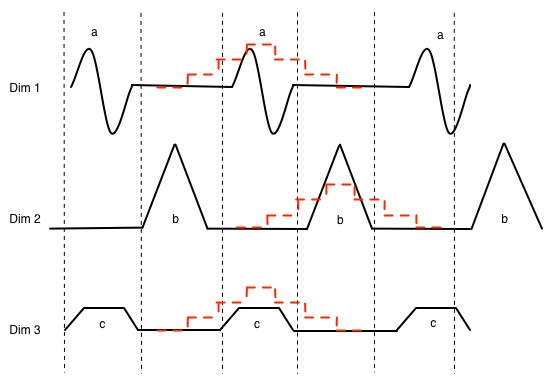
\includegraphics[scale=0.3]{MultiDimensionalMotif}
  \caption{Applying Guassian-resembled kernel function in multi dimensional motif discovery}
\end{figure}

% Definition of each parameter and the workflow of this algorithm
For each detected motif, assuming it starts from $A$ and ends with $B$. So the length of this motif is $B-A$. We extend the virtual 
length of each motif by spreading each side by $(B-A)/2$ therefore virtually the length of the motif becomes $2*(B-A)$ where it starts
with $(3*A-B)/2$ and ends with $(3*B-A)/2$. Suppose there are two motifs $M1$ with virtual length $ML1$ and $M2$ with virtual length
$ML2$ and we need to calculate how much $M1$ is co-occured with $M2$. Assume the number of window symbols they overlapped is $OVLP$, 
then the index of overlapping is calculated as:

\begin{center}
$ index = OVLP/ML2, index \in [0,1]$
\end{center}

And using the index here, we form the multi-dimensional motif collision table where each entry in the table represents 
how much one motif correlated with the other. A proper $threshold$, e.g. 0.5, should be picked carefully in filtering out the actual multi-dimensional motif.  

Assuming $NML$ is the list containing all merged motifs from different dimension that contains size $N$. $CM$ is the current motif being checked and $PM$ is the potential motif that might co-occured with $CM$, $INDEX(i,j)$ is the function to calculated the collision index of $motif i$ and $motif j$ as discussed above, $MMT$ is the Multi-dimensional Motif collision Table where each entry $MMT(i,j)$ represents how much $motif i$ correlated to $motif j$. 

The pseudocode for the algorithm is here
\begin{algorithm}
\caption{Forming MMT}
\begin{algorithmic}
\FOR{$i \in 1 \to N$}
\FOR{$j \in i+1 \to N$}
\IF{$NML(i) \cap NML(j)$}
\STATE $MMT(i,j) = MMT(i,j) + INDEX(i,j)$
\ENDIF
\ENDFOR
\ENDFOR
\STATE $MMT = MMT + transpose(MMT)$
\FOR{$k \in 1 \to N$}
\STATE $MMT(k,:) = MMT(k,:)/k.occ$
\ENDFOR
\end{algorithmic}
\end{algorithm}

% Graph for the multi-dimensional motif collision table
\begin{figure}
  \centering
  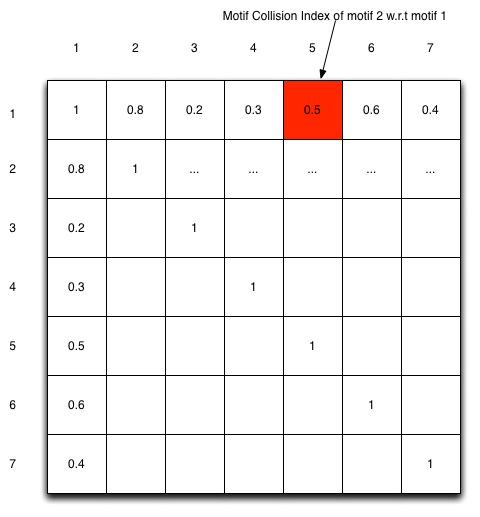
\includegraphics[scale=0.3]{MMT}
  \caption{Multi-dimensional Motif collision Table}
\end{figure}

Let the multi-dimensional motif(MDM) be a list that contains ids of the single dimension motif. 
Suppose the total number of motifs in all dimension is $N$.The multi-dimensional motif collision table (MMT) is a $N \times N$ matrix whose rows and cols are motif id arranged in ascending order. Each entry $MMT(i,j)$ represents the collision index of motif $i$ against motif $j$. Based on MMT. The pseudo code for the Edge-spreading Multi-dimensional Motif Detection(EMMD) algorithm. 

Here is pseudocode for the algorithm

\begin{algorithm}
\caption{EMMD}
\begin{algorithmic} 
\REQUIRE $threshold$
\STATE Output: MDM
\FOR {$i \in 1 \to  N$}
\STATE 	$ MDM \leftarrow MMT(i,:) > threshold$
\FOR{$\textbf{each} id \in MDM$}
\STATE $MMT(id,i) \leftarrow 0$
\STATE 	output $MDM$
\STATE 	$MDM \leftarrow \emptyset$
\ENDFOR
\ENDFOR
\end{algorithmic}
\end{algorithm}


\section{Experiment}


\section{Conclusion and Future Work}
Time series motif discovery has been proven to be a effective approach in activity and events detection. We have described an absolute unsupervised algorithm in discovering multi dimensional motifs in time varying data. The main contributions of our work are a bottom-top apprach to extract single dimensional motifs without manual configuration and a noise- tolerant multi dimensional motif discovery algorithm which are fundamental steps in conducting activity and event detection. The method is based on well known single dimensional motif discovery approach by \cite{Chiu03probabilisticdiscovery}. The unsupervised algorithm for single dimensional motif detection is based on the idea that long motifs can be represented as a sequence of short motifs. Multi dimensional motif detection algorithm has been improved by considering an edge-spreading linear kernel function in evaluating the correlation between motifs from different dimensions. In addition to evaluate our approach by synthetic data, we also use real life data produced by wearable body sensors. The results show that our approach can accurately detect the motifs in those sensor and thereby improved the event and activity recognition rate. For the future work, we will expolre the possibility of real-time multi-dimensional motif detection and deploy a real system that process and learn multi-dimensional motifs. 

\section{Illustrations}

Place all illustrations (figures, drawings, tables, and photographs)
throughout the paper at the places where they are first discussed,
rather than at the end of the paper. If placed at the bottom or top of
a page, illustrations may run across both columns.

Illustrations must be rendered electronically or scanned and placed
directly in your document. All illustrations should be in black and
white, as color illustrations may cause problems. Line weights should
be 1/2-point or thicker. Avoid screens and superimposing type on
patterns as these effects may not reproduce well.

Number illustrations sequentially. Use references of the following
form: Figure 1, Table 2, etc. Place illustration numbers and captions
under illustrations. Leave a margin of 1/4-inch around the area
covered by the illustration and caption.  Use 9-point type for
captions, labels, and other text in illustrations.

\section*{Acknowledgments}

The preparation of these instructions and the \LaTeX{} and Bib\TeX{}
files that implement them was supported by Schlumberger Palo Alto
Research, AT\&T Bell Laboratories, and Morgan Kaufmann Publishers.
Preparation of the Microsoft Word file was supported by IJCAI.  An
early version of this document was created by Shirley Jowell and Peter
F. Patel-Schneider.  It was subsequently modified by Jennifer
Ballentine and Thomas Dean, Bernhard Nebel, and Daniel Pagenstecher.
These instructions are the same as the ones for IJCAI--05, prepared by
Kurt Steinkraus, Massachusetts Institute of Technology, Computer
Science and Artificial Intelligence Lab.

\appendix

\section{\LaTeX{} and Word Style Files}\label{stylefiles}

The \LaTeX{} and Word style files are available on the IJCAI--13
website, {\tt http://www.ijcai-13.org/}.
These style files implement the formatting instructions in this
document.

The \LaTeX{} files are {\tt ijcai13.sty} and {\tt ijcai13.tex}, and
the Bib\TeX{} files are {\tt named.bst} and {\tt ijcai13.bib}. The
\LaTeX{} style file is for version 2e of \LaTeX{}, and the Bib\TeX{}
style file is for version 0.99c of Bib\TeX{} ({\em not} version
0.98i). The {\tt ijcai13.sty} file is the same as the {\tt
ijcai07.sty} file used for IJCAI--07.

The Microsoft Word style file consists of a single file, {\tt
ijcai13.doc}. This template is the same as the one used for
IJCAI--07.

These Microsoft Word and \LaTeX{} files contain the source of the
present document and may serve as a formatting sample.  

Further information on using these styles for the preparation of
papers for IJCAI--13 can be obtained by contacting {\tt
pcchair13@ijcai.org}.

%% The file named.bst is a bibliography style file for BibTeX 0.99c
\bibliographystyle{named}
\bibliography{momo_ijcai}

\end{document}

